\subsection{The Sedov Problem}\label{ss:sedov}

The dynamic problem of propagation of a blast wave in a $\gamma$-law compressible gas has been the focus of many researchers and has come to be known as the Sedov Problem.  The large bibliography of Sedov-studies may be summarized as in Griffiths (Chapter 10, Case Study: Taylor-Sedov Blast Wave) \cite{Griffiths} or Kamm and Timmes \cite{Kamm} and dates from the early work of Taylor \cite{Taylor} and von Neumann \cite{vonN} in 1941,  L.\  I.\  Sedov \cite{Sedov46} in 1946 (and 1959 \cite{Sedov}).

The results shown here are as defined in the last paragraph of Section 4.1 of Kamm and Timmes~ \cite{Kamm} for the geometry shown in Figure~\ref{fig:SedovGeom}.  Here, $H = 2 W$, $W = 1.25 \  \mathrm{cm}$, $D= 0.025 \ \mathrm{cm}$.  The mesh is constructed from hexahedra having  $\Delta x = \Delta y = \Delta z = W/50 = 0.025$ cm so that the mesh has 50 elements in the $X(1)$ direction, 100 in the $X(2)$ direction and 1 in the $X(3)$ direction.  Although the simulation is executed in a Cartesian system and because of the initial conditions being independent of $X(3)$, the problem becomes a two-dimensional Cylindrical geometry simulation.  Kamm and Timmes propose that for this case the stationary gas has $\gamma = 1.4$ and that at $t = 0$, the density is uniform at $\rho = 1$ gm/cc and that the blast total energy per unit depth is  $E_0 = 0.311357$ erg.  This value is such that at $t = 1\ s$ the blast wave will have a radius of $0.75$ cm.  Flexi requires initial values for density, momentum (x, y, z values) and pressure.  Consequently, since $ P = (\gamma - 1) \rho u$ and that initially with zero kinetic energy of the gas then $E_0/V_0 = \rho u$ and $V_0 = \pi R^2 Z$, where $Z$ is unit depth.  Then

\begin{eqnarray}
P_0 & = & (\gamma - 1) \frac{E_0 Z}{V_0} \\
   & = & (\gamma -1) \frac{E_0}{\pi R^2}  \nonumber \\
    & = & \frac{0.4 \ 0.311357}{ \pi\  0.025^2} \ \mathrm{dynes}/\mathrm{cm}^2 \nonumber \\
    & = & 63.43 \ \mathrm{dynes}/\mathrm{cm}^2 \nonumber
\end{eqnarray}
\noindent Outside of the blast zone, the intial pressure is set to $1. E -8$.

\begin{figure}[h!]
 \begin{center}
  \input{figures/Sedov-geom.pdf_t}
  \caption{The two-dimensional cylindrical Sedov problem geometry and mesh setup.}
  \label{fig:SedovGeom}
 \end{center}
\end{figure}

The two-dimensional initial pressure and final density ($t = 1.\ s$) fields are shown in Figure~\ref{fig:sedov2D} and for comparison to exact results the extracted line plots for this simulation are presented in Figures~\ref{fig:CVsedov} and \ref{fig:PVsedov}.  The line plots are along a $45^o$ ray from the origin into the first quardant.  Flexi mesh and input files are listed in \ref{ssec:hoprin-sedov} and \ref{ssec:flexiin-sedov}.  In the Flexi input file, note that the value of $\mathrm{IniExactFunc} = 1342$ and $\mathrm{eradius\_in} = 0.025$.  This is a special exact function coded into flexi/src/equations/navierstokes/idealgas/exactfunc.f90 which specifies that if $X(1)^2 + X(2)^2 \ge \mathrm{eradius}$\_$\mathrm{in}^2$ for all $X(3)$ then RefState 1 applies, otherwise RefState 2 applies.  The Flexi results were extracted from ParaView at $t = 1.\ s$ using the plotOverLine app, with the line running from $(0,0,-0.0125)$ to $(1.25, 1.25, -0.0125)$.

\begin{figure}[h!]
\centering
\begin{subfigure}[h!]{0.9\linewidth}
\centering
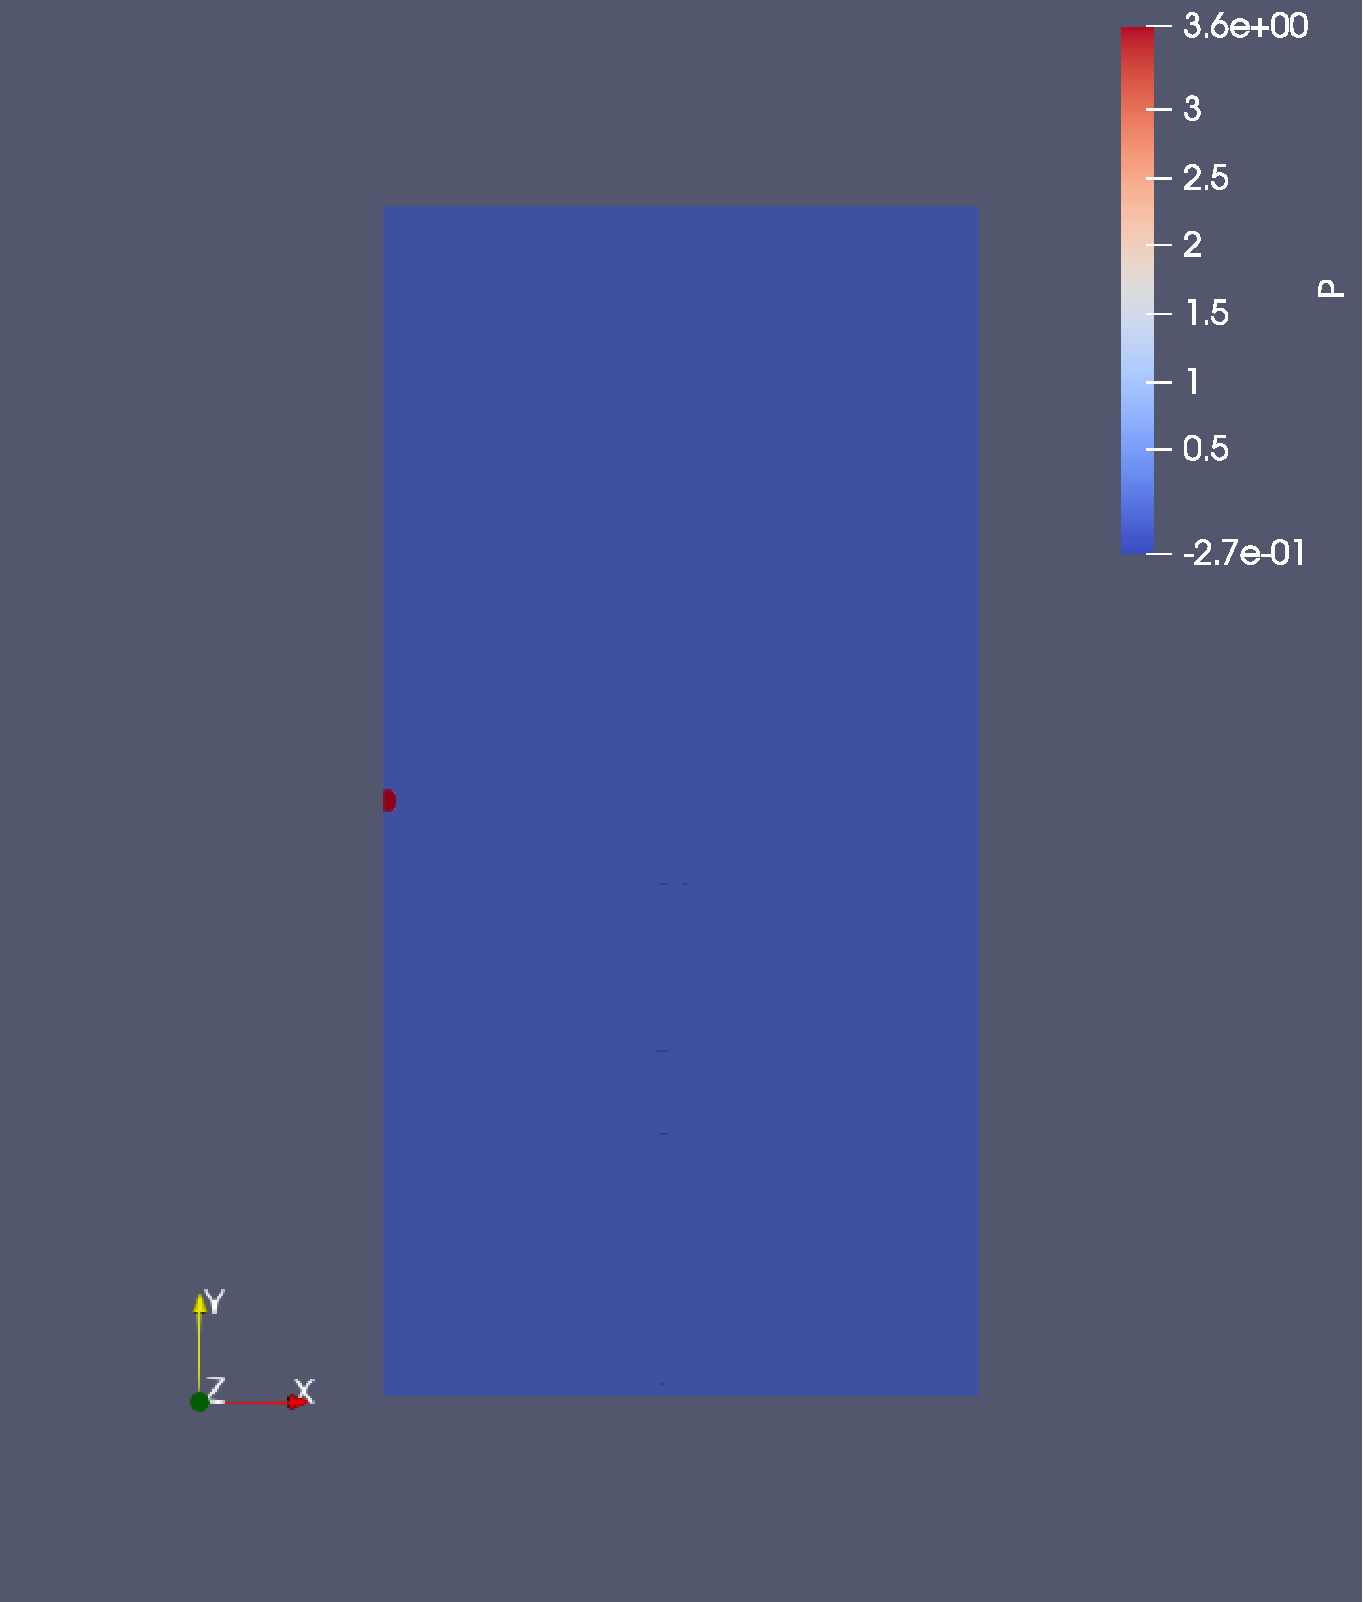
\includegraphics[scale=0.25]{figures/sedov-00-P.pdf }
\caption{Initial pressure field for the Sedov problem showing the small (2 element) region of initially high pressure.\bigskip \bigskip}
  \label{fig:sedov-0}
\end{subfigure}

\begin{subfigure}[h!]{0.9\linewidth}
\centering
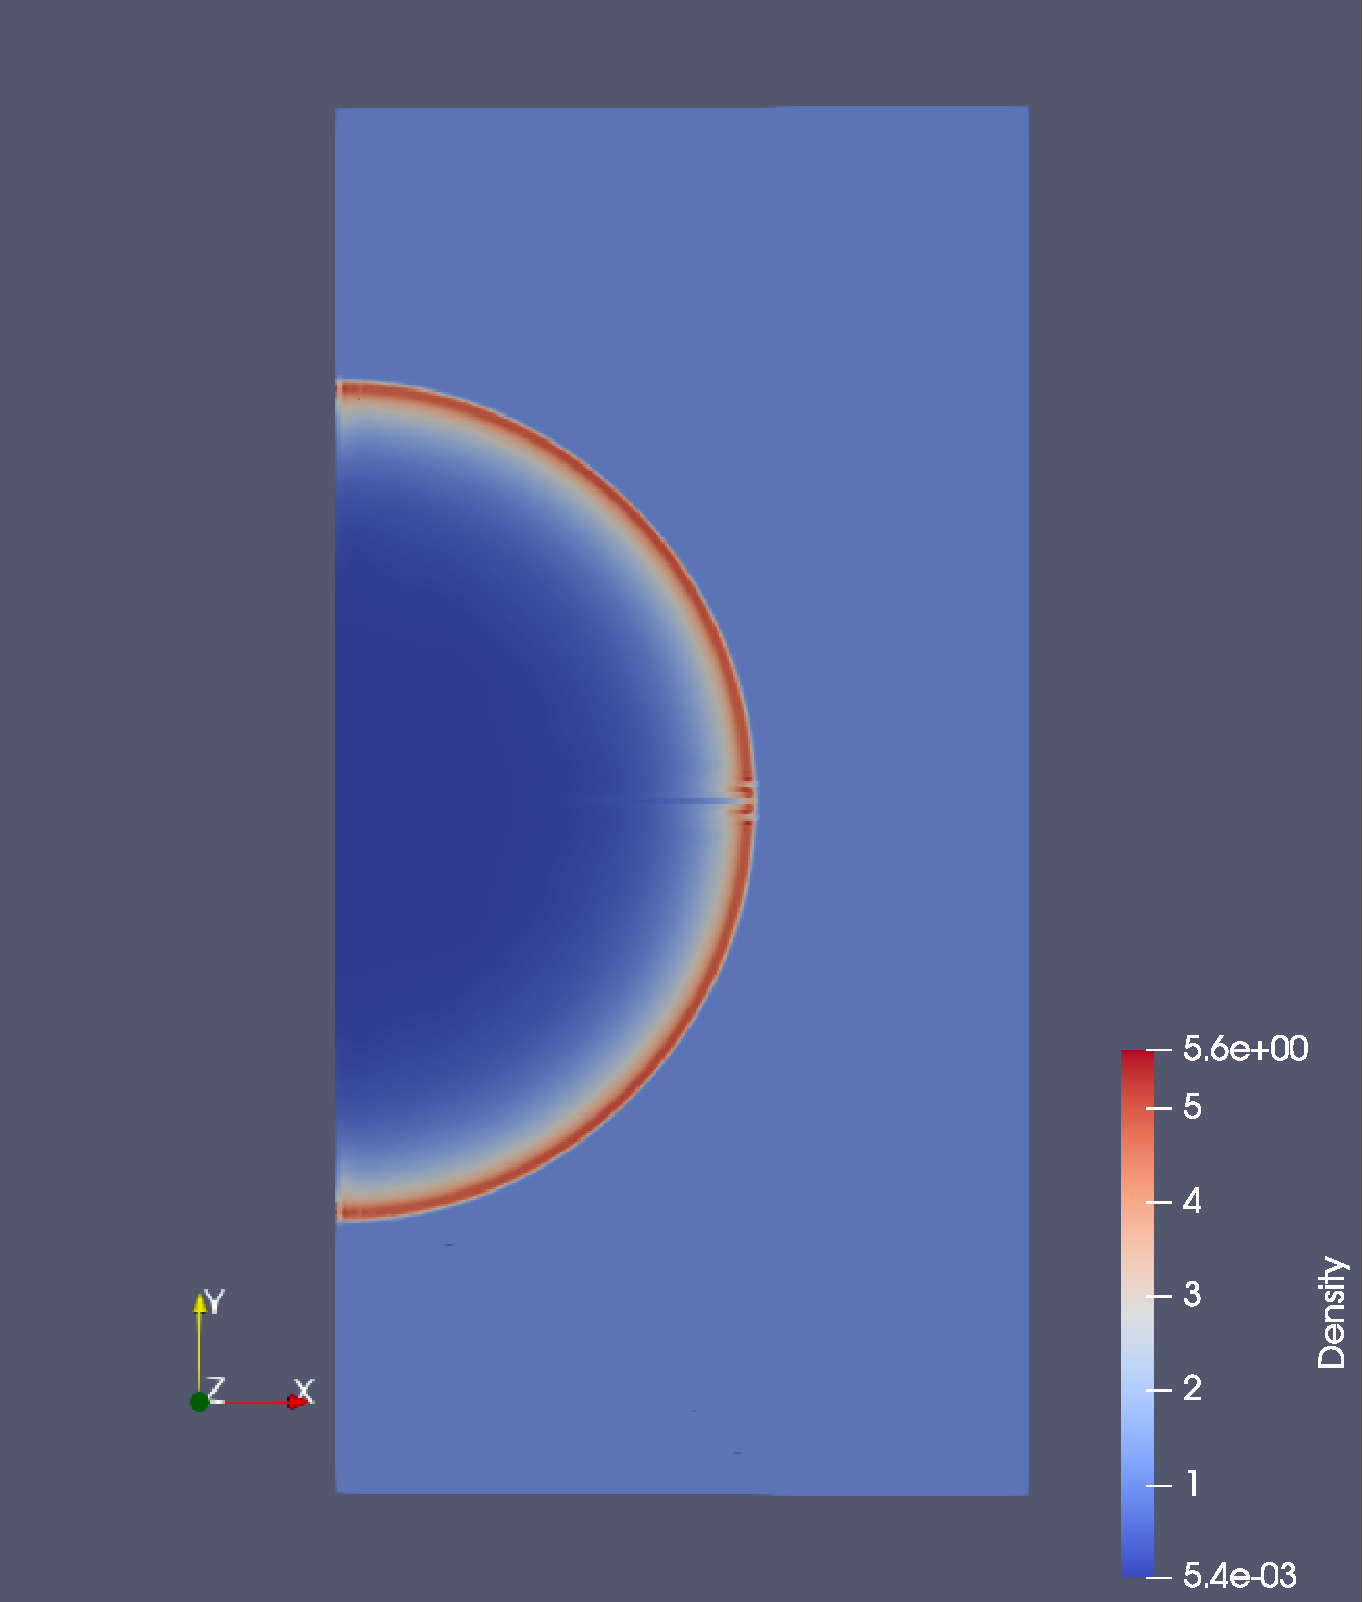
\includegraphics[scale=0.25]{figures/sedov-10-den.pdf }
\caption{Final $t = 1. \  s$ density field for the Sedov problem. Some minor irregularities are shown at the shock front along both the x and y-axes. However the shock front arrives at a radius very close to $R = 0.75$ as expected.}
  \label{fig:sedov-10}
\end{subfigure}
\caption{The Sedov problem results for the density field.}
\label{fig:sedov2D}
\end{figure}

\begin{figure}[h!]
 \centering
 \includegraphics[scale=0.8]{figures/sedov-CV.pdf}
 \caption{Sedov problem at $t = 1.\ s$ and showing the conserved variables.  Comparison is made to the exact solution (in blue.) }
 \label{fig:CVsedov}
\end{figure}

\begin{figure}[h!]
 \centering
 \includegraphics[scale=0.8]{figures/sedov-PV.pdf}
 \caption{Sedov problem at $t = 1. \ s$, showing primitive variables.  Comparison is made to the exact solution (in blue.)}
 \label{fig:PVsedov}
\end{figure}

\noindent It is noted that the shock arrives very close to a radius of $0.75$ at $t = 1.\ s$  Table~\ref{tab:sedovEps} shows the average error in the Flexi solution to be less than $5.7E-3$ except for specific internal energy.

\begin{table}[h!]
 \centering
 \begin{tabular}{|c|c|} \hline
   Variable & $\bar{\epsilon}$ \\ \hline \hline
   $\rho$ & 5.62E-3\\
   $|m_i|$  & 3.33E-3 \\
   $E$      & 1.97 E-3 \\ \hline
   $|v_i|$  & 1.8988E-3 \\
   $u$     & 1.86E-1 \\
   $P$     & 9.86865E-4 \\ \hline
 \end{tabular}
 \caption{Average error (\textit{c.f.,} Eq.~\ref{eq:error}) for the Sedov Problem}\label{tab:sedovEps}
\end{table}

The exact solutions presented for the Sedov Problem were computed using the Sedov solver in ExactPack \cite{exactpack}, a newly released Python3 package designed specfically to be used as code verification.  It is available from \url{https://github.com/lanl/ExactPack}.  The Doebling Sedov solver was modified to compute conserved variables and to print out exact solution data files.

\paragraph{Conclusions}
These results show a very good agreement between Flexi and exact results for this challenging two-dimensional problem.
